\documentclass[aspectratio=169]{beamer}

\usepackage{babel}
\usepackage{xcolor}
\usepackage{mathtools}
\usepackage{amsfonts}
\usepackage{bm}

% Iverson brackets.
\DeclareFontFamily{U}{matha}{\hyphenchar\font45}
\DeclareFontShape{U}{matha}{m}{n}{ <-6> matha5 <6-7> matha6 <7-8>
matha7 <8-9> matha8 <9-10> matha9 <10-12> matha10 <12-> matha12 }{}
\DeclareSymbolFont{matha}{U}{matha}{m}{n}
\DeclareFontFamily{U}{mathx}{\hyphenchar\font45}
\DeclareFontShape{U}{mathx}{m}{n}{ <-6> mathx5 <6-7> mathx6 <7-8>
mathx7 <8-9> mathx8 <9-10> mathx9 <10-12> mathx10 <12-> mathx12 }{}
\DeclareSymbolFont{mathx}{U}{mathx}{m}{n}
\DeclareMathDelimiter{\liv} {4}{matha}{"76}{mathx}{"30}
\DeclareMathDelimiter{\riv} {5}{matha}{"77}{mathx}{"38}

\usetheme{default}
\usefonttheme{serif}

% Chess!
\usepackage{chessboard}
\storechessboardstyle{nqueens}{%
  maxfield=e5,
  clearboard,
  setpieces={Qa2, Qb5, Qc3, Qd1, Qe4},
  showmover=false,
  color=boxblue, fieldcolor=boxblue!50!black,
  setfontcolors=boxblue, addfontcolors,
  labelleftformat={\color{boxblue}\arabic{ranklabel}},
  labelbottomformat={\color{boxblue}\arabic{filelabel}}
}

% Tables.
\usepackage{multirow}

% Bibliography.
\usepackage{natbib}
\usepackage{bibentry}
\bibliographystyle{plainnat}

% Colors
\definecolor{palette-orange}{HTML}{ff3a20}
\definecolor{palette-green}{HTML}{5b8c5a}
\definecolor{palette-blue}{HTML}{0e79b2}
\definecolor{palette-yellow}{HTML}{f5b700}
\definecolor{palette-dgreen}{HTML}{1e2f23}
\definecolor{palette-purple}{HTML}{331832}
\definecolor{dark gray}{HTML}{808080}
\definecolor{darker gray}{HTML}{606060}

\definecolor{alt-palette1}{HTML}{003049}
\definecolor{alt-palette2}{HTML}{a62639}
\definecolor{alt-palette3}{HTML}{f77f00}
\definecolor{alt-palette4}{HTML}{3bb273}
\definecolor{alt-palette5}{HTML}{4d9de0}
\definecolor{alt-palette6}{HTML}{d7cf07}
\definecolor{alt-palette7}{HTML}{97b1a6}
\definecolor{alt-palette8}{HTML}{386641}

\definecolor{palette1}{HTML}{FFBE0B}
\definecolor{palette2}{HTML}{FB5607}
\definecolor{palette3}{HTML}{FF006E}
\definecolor{palette4}{HTML}{8338EC}
\definecolor{palette5}{HTML}{3A86FF}
\definecolor{palette6}{HTML}{b2ef9b}
\definecolor{palette7}{HTML}{2e294e}
\definecolor{palette8}{HTML}{2c0703}
\definecolor{palette9}{HTML}{e2cfea}

% Old colors
\definecolor{boxgray}{HTML}{808080}
\definecolor{boxdgray}{HTML}{545454}
\definecolor{boxnteal}{HTML}{467085}
\definecolor{boxdgreen}{HTML}{335C33}
\definecolor{boxbrown}{HTML}{4C331A}
\definecolor{boxkpgreen}{HTML}{3beb7e}

\definecolor{boxblue}{HTML}{3275a8}
\definecolor{boxlblue}{HTML}{AFDCFF}
\definecolor{boxorange}{HTML}{ce654f}
\definecolor{boxlorange}{HTML}{cc7d6d}
\definecolor{boxllorange}{HTML}{edaea1}
\definecolor{boxpurple}{HTML}{271F36}
\definecolor{boxred}{HTML}{B44650}
\definecolor{boxgreen}{HTML}{54774B}
\definecolor{boxlgreen}{HTML}{9CD08F}
\definecolor{boxteal}{HTML}{568777}
\definecolor{boxlteal}{HTML}{88C7B2}
\definecolor{boxgold}{HTML}{EFA906}
\definecolor{boxdyellow}{HTML}{F9CB40}
\definecolor{boxgoldenrod}{HTML}{818a34}
\definecolor{boxpink}{HTML}{b522a4}
\definecolor{boxwheat}{HTML}{e1ca96}
\definecolor{boxolive}{HTML}{bbbe64}
\definecolor{boxmunsel}{HTML}{04a777}

\definecolor{pviolet}{HTML}{8332AC}
\definecolor{psandy}{HTML}{6C441E}
\definecolor{pdgreen}{HTML}{219E31}
\definecolor{pbrickred}{HTML}{D1495B}
\definecolor{pyellow}{HTML}{FFE066}

\definecolor{rightgreen}{HTML}{54774B}
\definecolor{wrongred}{HTML}{B44650}

% dPASP
\newcommand{\dpasp}{\textbf{\textcolor{palette-purple}{$\bm{d}$}\,\textcolor{palette-orange}{$\pmb{\mathbb{P}}$}\textcolor{palette-green}{A}\textcolor{palette-blue}{S}\textcolor{palette-yellow}{P}}}
\newcommand{\dpaspnc}{\textbf{$\bm{d}$\,$\pmb{\mathbb{P}}$ASP}}
% PASP
\newcommand{\paspc}{\textbf{\textcolor{palette-orange}{$\pmb{\mathbb{P}}$}\textcolor{palette-green}{A}\textcolor{palette-blue}{S}\textcolor{palette-yellow}{P}}}
\newcommand{\paspnc}{\textbf{$\pmb{\mathbb{P}}$ASP}}
% ASP
\newcommand{\aspc}{\textbf{\textcolor{palette-green}{A}\textcolor{palette-blue}{S}\textcolor{palette-yellow}{P}}}
\newcommand{\aspnc}{\textbf{ASP}}

% Inline images.
\newcommand{\inlineimg}[1]{\raisebox{-.25\height}{\includegraphics[height=1em]{figures/#1}}}


% Check marks
\usepackage{pifont}
\newcommand{\cmark}{\color{rightgreen}\ding{51}}%
\newcommand{\xmark}{\color{wrongred}\ding{55}}%
\newcommand{\omark}{{\color{dark gray}\tiny$\bm{\circ}$}}%
\newcommand{\done}{\rlap{$\square$}{\raisebox{2pt}{\large\hspace{1pt}\cmark}}}
\newcommand{\wontfix}{\rlap{$\square$}{\large\hspace{1pt}\xmark}}

% Source code
\usepackage{times}
\usepackage{soul}
\usepackage{inconsolata}
\usepackage{minted}
\definecolor{mintedframe}{HTML}{5ca4a9}
\setminted{
    fontsize=\small,
    escapeinside=&&,
    rulecolor=mintedframe,
}
\usemintedstyle{sas}
\newminted[pasp]{pasp}{mathescape}
\newmintinline[paspi]{pasp}{mathescape}
\newmintinline[paspin]{pasp}{mathescape,fontsize=\LARGE}
\newmintedfile[paspf]{pasp}{mathescape}

\usepackage{tikz}
\usetikzlibrary{shapes}
\usetikzlibrary{shapes.multipart}
\usetikzlibrary{fit}
\usetikzlibrary{decorations.pathreplacing,calligraphy,calc}
\usetikzlibrary{arrows.meta,matrix,arrows}
\usetikzlibrary{positioning,circuits.logic.US,shadows,shadings,shapes.symbols,backgrounds}

\newcommand{\ccimg}{%
  \hspace{0.25cm}\def\svgwidth{0.1\textwidth}\input{figures/cc.pdf_tex}%
}

\usepackage{pgfplots}
\pgfplotsset{compat=1.18}

% Circuits
\newcommand{\newGraphNode}[4]{\node[#4] (#1) at (#2) {\rotatebox{-90}{#3}}}
\newcommand{\newNamedAndNode}[4][]{\node[#1,and gate,fill=blue!50!red!30,inner sep=0pt,scale=0.75,minimum size=12pt,thick,rotate=89.9,#1] (#2) at (#3) {\rotatebox{-90}{#4}}}
\newcommand{\newNamedOrNode}[4][]{\node[#1,or gate,fill=blue!50!green!30,inner sep=0pt,scale=0.75,minimum size=12pt,thick,rotate=89.9,#1] (#2) at (#3) {\rotatebox{-90}{#4}}}
\newcommand{\newAndNode}[3][]{\node[#1,and gate,fill=blue!50!red!30,thick,inner sep=0pt,scale=0.75,minimum size=12pt,rotate=89.9,#1] (#2) at (#3) {}}
\newcommand{\newOrNode}[3][]{\node[#1,or gate,fill=blue!50!green!30,thick,inner sep=0pt,scale=0.75,minimum size=12pt,rotate=89.9,#1] (#2) at (#3) {}}
\newcommand{\newLitNode}[4][]{\node[#1,minimum size=17pt,label=center:{#4}] (#2) at (#3) {}}
\tikzset{
  circuit logic US,tips=proper,edge/.style = {->,>=latex'},
}

\newcommand{\newSumNode}[3][]{\node[circle,draw,inner sep=0pt,minimum size=12pt,thick,fill=blue!50!green!30,#1] (#2) at (#3) {$\bm{+}$}}
\newcommand{\newMaxNode}[3][]{\node[circle,draw,inner sep=0pt,minimum size=12pt,thick,fill=blue!50!green!30,#1] (#2) at (#3) {\scriptsize$\bm{\uparrow}$}}
\newcommand{\newMixNode}[3][]{\node[#1,circle,draw,inner sep=0pt,minimum size=12pt,thick,fill=blue!50!green!30] (#2) at (#3) {$\sum$}}
\newcommand{\newProdNode}[3][]{\node[circle,draw,inner sep=0pt,minimum size=12pt,thick,fill=blue!50!red!30,#1] (#2) at (#3) {$\bm{\times}$}}
\newcommand{\newLeafNode}[3][]{\node[circle,draw,inner sep=0pt,minimum
size=12pt,thick,fill=orange!50!black!40,#1] (#2) at (#3) {}; \node[circle,draw,inner sep=0pt,minimum size=5pt,line width=0.6pt] at (#3) {}}
\newcommand{\newCellNode}[3][]{\node[#1,circle,draw,inner sep=0pt,minimum size=12pt,thick,fill=orange!50!black!40] (#2) at (#3) {$\bm{\Box}$}}
\tikzset{sigmoid/.style={path picture={\begin{scope}[x=0.65pt,y=7pt] \draw plot[domain=-6:6](\x,{1/(1+exp(-1.5*\x))-0.5}); \end{scope}}}}
\tikzset{gaussian/.style={path picture={\begin{scope}[x=1pt,y=10pt] \draw plot[domain=-4:4](\x,{exp(-\x*\x*0.5)/2.5-0.1}); \end{scope}}}}
\newcommand{\newProjNode}[3][]{\node[#1,sigmoid,circle,draw,inner sep=2pt,minimum size=13pt,thick,fill=blue!50!green!30] (#2) at (#3) {};}
\newcommand{\newGaussNode}[3][]{\node[gaussian,circle,draw,inner sep=2pt,minimum size=13pt,thick,fill=orange!50!black!40,#1] (#2) at (#3) {};}
\newcommand{\newPartNode}[3][]{\node[#1,circle split,rotate=90,draw,inner sep=2pt,minimum size=12pt,thick,fill=blue!50!red!30] (#2) at (#3) {};}
\newcommand{\inode}[2][]{\tikz[baseline=-0.75ex]{#2[scale=0.8,#1]{r}{0,0};}}
\newcommand{\newVtreeNode}[4][]{\node[#1,draw,inner sep=2pt,minimum size=13pt] (#2) at (#3) {#4}}

% Gaussians.
\usepgfplotslibrary{fillbetween}
\pgfmathdeclarefunction{gauss}{2}{%
  \pgfmathparse{1/(#2*2.5066)*exp(-((x-#1)^2)/(2*#2^2))}%
}
\pgfmathdeclarefunction{egauss}{3}{%
  \pgfmathparse{1/(#2*2.5066)*exp(-((#3-#1)^2)/(2*#2^2))}%
}
\pgfmathdeclarefunction{gauss3}{6}{%
  \pgfmathparse{(exp(-((x-#1)^2)/(2*#2^2))/#2+exp(-((x-#3)^2)/(2*#4^2))/#4+exp(-((x-#5)^2)/(2*#6^2))/#6)/2.5066}%
}
\pgfmathdeclarefunction{mixgauss3}{9}{%
  \pgfmathparse{(#7*exp(-((x-#1)^2)/(2*#2^2))/#2+#8*exp(-((x-#3)^2)/(2*#4^2))/#4+#9*exp(-((x-#5)^2)/(2*#6^2))/#6)/2.5066}%
}
\pgfmathdeclarefunction{mixgauss3t}{9}{%
  \pgfmathparse{((x < 1.25) ? #7*egauss(#1, #2, x) : ((x < 3.25) ? #8*egauss(#3, #4, x) : #9*egauss(#5, #6, x)))/0.7574}%
}
\pgfmathdeclarefunction{mixgauss2}{6}{%
  \pgfmathparse{(#5*exp(-((x-#1)^2)/(2*#2^2))/#2+#6*exp(-((x-#3)^2)/(2*#4^2))/#4)/2.5066}%
}
\pgfmathdeclarefunction{mixgauss2y}{6}{%
  \pgfmathparse{(#5*exp(-((y-#1)^2)/(2*#2^2))/#2+#6*exp(-((y-#3)^2)/(2*#4^2))/#4)/2.5066}%
}

% Circles and intersection tools.
\newcommand{\logiccircle}{(1.25,-1.25) circle (2)}
\newcommand{\probcircle}{(-1.25,-1.25) circle (2)}
\newcommand{\neuralcircle}{(0,1.25) circle (2)}
\newcommand{\complrect}{(-3.5,-3.5) rectangle (3.5, 3.5)}
\newcommand{\logicpoint}{(1.25,-1.25)}
\newcommand{\probpoint}{(-1.25,-1.25)}
\newcommand{\neuralpoint}{(0,1.25)}

% Vertical and horizontal centering.
\newenvironment{vhcenterb}{\vspace*{\fill}\begin{center}}{\end{center}\vspace*{\fill}}

%%%%%%%%%%%%%%%%%%%%%%%%%%%%%%%%%%%%%%% END OF PREAMBLE %%%%%%%%%%%%%%%%%%%%%%%%%%%%%%%%%%%%%%%%%%%

\author{\small\textbf{Renato Lui Geh}, Jonas Gonçalves, Igor Cataneo Silveira,\texorpdfstring{\\}{
}Denis Deratani Mauá, Fabio Gagliardi Cozman, Yuka Machino}
\subtitle{\texorpdfstring{\color{black}\large{}}{}Programming with Logic and Neural Networks}
\date{}

\makeatletter
\setbeamertemplate{title page}[default][left]
\makeatother

\begin{document}

\title{\rmfamily\bfseries\Huge\dpasp}

%%%%%%%%%%%%%%%%%%%%%%%%%%%%%%%%%%%%%%%%%%%%%%%%%%%%%%%%%%%%%%%%%%%%%%%%%%%%%%%%%%%%%%%%%%%%%%%%%%%

\begin{frame}
    \titlepage
    \ccimg
\end{frame}

%%%%%%%%%%%%%%%%%%%%%%%%%%%%%%%%%%%%%%%%%%%%%%%%%%%%%%%%%%%%%%%%%%%%%%%%%%%%%%%%%%%%%%%%%%%%%%%%%%%

\newcommand{\dpaspslide}[1]{
\setbeamercolor{frametitle}{bg=palette-yellow,fg=white}
\begin{frame}{\textbf{$\bm{d}\,\pmb{\mathbb{P}}$ASP for Neurosymbolic Learning and Reasoning}}
\centering
\begin{tikzpicture}
  \onslide<1>{
    \node (neural) at (0, 1.25) {};
    \node (prob) at (-1.25, -1.25) {};
    \node (logic) at (1.25, -1.25) {};
    \fill[palette-blue,opacity=0.6] (neural) circle (2);
    \fill[palette-green,opacity=0.6] (prob) circle (2);
    \fill[palette-orange,opacity=0.6] (logic) circle (2);
    \draw[thick] (neural) circle (2) node[yshift=0.5cm,opacity=1.0] {\sf\LARGE\color{white}\textbf{Neural}};
    \draw[thick] (prob) circle (2) node[xshift=-0.7cm,yshift=-0.15cm,opacity=1.0] {\sf\LARGE\color{white}\textbf{Prob}};
    \draw[thick] (logic) circle (2) node[xshift=0.7cm,yshift=-0.15cm,opacity=1.0] {\sf\LARGE\color{white}\textbf{Logic}};
  }
  \ifnum#1=1
  \onslide<2->{
    \node (neural) at (0, 1.25) {};
    \node (prob) at (-1.25, -1.25) {};
    \node (logic) at (1.25, -1.25) {};
    \fill[palette-blue,opacity=0.1] (neural) circle (2);
    \fill[palette-green,opacity=0.1] (prob) circle (2);
    \fill[palette-orange,opacity=0.1] (logic) circle (2);
    \draw[opacity=0.1,thick] (neural) circle (2) node[yshift=0.5cm,opacity=1.0] {\sf\LARGE\color{white}\textbf{Neural}};
    \draw[opacity=0.1,thick] (prob) circle (2) node[xshift=-0.7cm,yshift=-0.15cm,opacity=1.0] {\sf\LARGE\color{white}\textbf{Prob}};
    \draw[opacity=0.1,thick] (logic) circle (2) node[xshift=0.7cm,yshift=-0.15cm,opacity=1.0] {\sf\LARGE\color{white}\textbf{Logic}};
    \scope
    \clip (neural) circle (2);
    \clip (logic) circle (2);
    \fill[palette-yellow] (prob) circle (2);
    \draw[very thick] (prob) circle (2);
    \endscope
    \scope
    \clip (prob) circle (2);
    \clip (logic) circle (2);
    \draw[very thick] (neural) circle (2);
    \endscope
    \scope
    \clip (prob) circle (2);
    \clip (neural) circle (2);
    \draw[very thick] (logic) circle (2);
    \endscope
    \node[yshift=-1.25cm] at (0, 0) {\LARGE\textbf{\textcolor{palette-purple}{$\bm{d}$}\,\textcolor{palette-orange}{$\pmb{\mathbb{P}}$}\textcolor{palette-green}{A}\textcolor{palette-blue}{S}\textcolor{palette-yellow}{P}}};
  }
  \fi
  \ifnum#1=2
  \onslide<2->{
    \node (neural) at (0, 1.25) {};
    \node (prob) at (-1.25, -1.25) {};
    \node (logic) at (1.25, -1.25) {};
    \fill[palette-blue,opacity=0.1] (neural) circle (2);
    \fill[palette-green,opacity=0.1] (prob) circle (2);
    \fill[palette-orange,opacity=0.1] (logic) circle (2);
    \draw[opacity=0.1,thick] (neural) circle (2) node[yshift=0.5cm,opacity=1.0] {\sf\LARGE\color{white}\textbf{Neural}};
    \draw[opacity=0.1,thick] (prob) circle (2) node[xshift=-0.7cm,yshift=-0.15cm,opacity=1.0] {\sf\LARGE\color{white}\textbf{Prob}};
    \begin{scope}[even odd rule]
      \clip \neuralcircle \complrect;
      \clip \probcircle \complrect;
      \fill[opacity=0.6,palette-orange] \logiccircle;
      \draw[thick] \logiccircle;
    \end{scope}
    \begin{scope}[even odd rule]
      \clip \neuralcircle \complrect;
      \clip \logiccircle;
      \draw[thick] \probcircle;
    \end{scope}
    \begin{scope}[even odd rule]
      \clip \probcircle \complrect;
      \clip \logiccircle;
      \draw[thick] \neuralcircle;
    \end{scope}
    \onslide<2>{
      \draw[opacity=0.1,thick] (logic) circle (2) node[xshift=0.7cm,yshift=-0.15cm,opacity=1.0] {\sf\LARGE\color{white}\textbf{Logic}};
    }
    \onslide<3>{
      \draw[opacity=0.1,thick] (logic) circle (2) node[xshift=0.7cm,yshift=-0.15cm,opacity=1.0] {\sf\LARGE\color{white}\textbf{LP}};
    }
  }
  \fi
  \ifnum#1=3
  \onslide<2->{
    \node (neural) at (0, 1.25) {};
    \node (prob) at (-1.25, -1.25) {};
    \node (logic) at (1.25, -1.25) {};
    \fill[palette-blue,opacity=0.1] (neural) circle (2);
    \fill[palette-green,opacity=0.1] (prob) circle (2);
    \fill[palette-orange,opacity=0.1] (logic) circle (2);
    \draw[opacity=0.1,thick] (neural) circle (2) node[yshift=0.5cm,opacity=1.0] {\sf\LARGE\color{white}\textbf{Neural}};
    \begin{scope}[even odd rule]
      \clip \neuralcircle \complrect;
      \fill[opacity=0.6,palette-green] \probcircle;
    \end{scope}
    \begin{scope}[even odd rule]
      \clip \neuralcircle \complrect;
      \fill[opacity=0.6,palette-orange] \logiccircle;
    \end{scope}
    \begin{scope}[even odd rule]
      \clip \neuralcircle \complrect;
      \draw[thick] \logiccircle;
    \end{scope}
    \begin{scope}[even odd rule]
      \clip \logiccircle;
      \draw[thick] \neuralcircle;
    \end{scope}
    \begin{scope}[even odd rule]
      \clip \neuralcircle \complrect;
      \draw[thick] \probcircle;
    \end{scope}
    \begin{scope}[even odd rule]
      \clip \probcircle;
      \draw[thick] \neuralcircle;
    \end{scope}
    \draw[opacity=0.1,thick] \logiccircle node[xshift=0.7cm,yshift=-0.15cm,opacity=1.0] {\sf\LARGE\color{white}\textbf{LP}};
    \draw[opacity=0.1,thick] \probcircle node[xshift=-0.7cm,yshift=-0.15cm,opacity=1.0] {\sf\LARGE\color{white}\textbf{PL}};
    \onslide<3>{
      \path \logicpoint -- \probpoint node[midway,below=2cm] {\sf\LARGE\paspc{}};
      \path \logicpoint -- \probpoint node[midway,yshift=-0.15cm] {\sf\LARGE\color{white}\textbf{PLP}};
    }
  }
  \fi
\end{tikzpicture}
\end{frame}
}

%%%%%%%%%%%%%%%%%%%%%%%%%%%%%%%%%%%%%%%%%%%%%%%%%%%%%%%%%%%%%%%%%%%%%%%%%%%%%%%%%%%%%%%%%%%%%%%%%%%

\dpaspslide{1}

%%%%%%%%%%%%%%%%%%%%%%%%%%%%%%%%%%%%%%%%%%%%%%%%%%%%%%%%%%%%%%%%%%%%%%%%%%%%%%%%%%%%%%%%%%%%%%%%%%%

\dpaspslide{2}

%%%%%%%%%%%%%%%%%%%%%%%%%%%%%%%%%%%%%%%%%%%%%%%%%%%%%%%%%%%%%%%%%%%%%%%%%%%%%%%%%%%%%%%%%%%%%%%%%%%

\setbeamercolor{frametitle}{bg=palette-orange,fg=white}
\begin{frame}{\textbf{Horn Logic}}
\begin{vhcenterb}
  \includegraphics[width=2cm]{figures/horn.jpg}\\
  {\scriptsize Alfred Horn (1918 -- 2001)}

  \vspace{0.25cm}
  \textcolor{palette-blue}{\textbf{A\only<3>{n} \underline{\only<1>{rule}\only<2>{fact}\only<3>{integrity constraint}} is...}}
  \vspace{0.1cm}
  \begin{equation*}
    \only<1,3>{(\neg b_1\vee\neg b_2\vee\cdots\vee\neg b_n)}\only<2>{\top}
    \vee \only<1,2>{(h_1\vee h_2\vee\cdots\vee h_m)}\only<3>{\bot}
  \end{equation*}
  \begin{equation*}
                                              \equiv
  \end{equation*}
  \begin{equation*}
    \underbrace{\only<1,2>{h_1\vee h_2\vee\cdots\vee h_m}\only<3>{\bot}}_{\text{Head}}\gets
    \underbrace{\only<1,3>{b_1\wedge b_2\wedge\cdots\wedge b_n}\only<2>{\top}}_{\text{Body}}.
  \end{equation*}
  \vspace*{0.2cm}

  \textcolor{boxdgreen}{\textbf{Intuition:} \only<1>{\emph{if} $b_1\wedge\cdots\wedge b_n$, \emph{then}
  one of $h_1,\cdots,h_m$ must hold.}\only<2>{$h_1,\cdots,h_m$ are \emph{always} true.}
  \only<3>{$b_1\wedge\cdots\wedge b_n$ \emph{cannot} be true.}}
\end{vhcenterb}

\textcolor{dark gray}{\scriptsize\citep{horn51}}
\end{frame}

%%%%%%%%%%%%%%%%%%%%%%%%%%%%%%%%%%%%%%%%%%%%%%%%%%%%%%%%%%%%%%%%%%%%%%%%%%%%%%%%%%%%%%%%%%%%%%%%%%%

\setbeamercolor{frametitle}{bg=palette-orange,fg=white}
\begin{frame}[fragile]{\textbf{Answer Set Programming}}
\begin{minipage}{0.6\textwidth}
  \begin{minted}[fontsize=\footnotesize]{pasp}
% Solving Towers of Hanoi with ASP.

{ move(D,P,T) : disk(D), peg(P) } = 1 :- moves(M), T = 1..M.

move(D,T)   :- move(D,_,T).
on(D,P,0)   :- init_on(D,P).
on(D,P,T)   :- move(D,P,T).
on(D,P,T+1) :- on(D,P,T), not move(D,T+1),
                          not moves(T).
blocked(D-1,P,T+1) :- on(D,P,T), not moves(T).
blocked(D-1,P,T)   :- blocked(D,P,T), disk(D).

:- move(D,P,T), blocked(D-1,P,T).
:- move(D,T), on(D,P,T-1), blocked(D,P,T).
:- goal_on(D,P), not on(D,P,M), moves(M).
:- { on(D,P,T) } != 1, disk(D), moves(M), T = 1..M.
  \end{minted}
\end{minipage}%
\begin{minipage}{0.4\textwidth}
  \resizebox{\textwidth}{!}{
  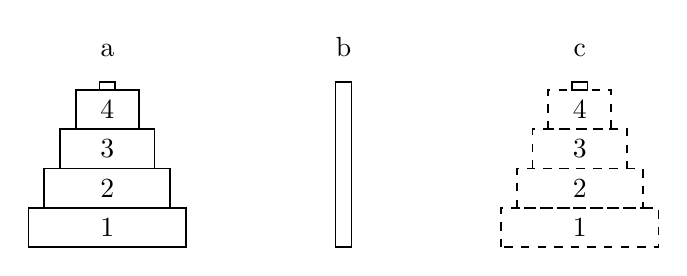
\begin{tikzpicture}[->,>=stealth',semithick]
		% peg a 0.0 - 3.0
		\draw (0.5,0)   rectangle node {1} (2.5,0.5);
		\draw (0.7,0.5) rectangle node {2} (2.3,1);
		\draw (0.9,1)   rectangle node {3} (2.1,1.5);
		\draw (1.1,1.5) rectangle node {4} (1.9,2);
		\draw (1.4,2)   rectangle          (1.6,2.1);
		\draw [-] (1.5,2.3) node [above] {a};
		% peg b 3.0 - 6.0
		\draw (4.4,0.0)   rectangle          (4.6,2.1);
		\draw [-] (4.5,2.3) node [above] {b};
		% peg c 6.0 - 9.0
		\draw [dashed] (6.5,0)   rectangle node {1} (8.5,0.5);
		\draw [dashed] (6.7,0.5) rectangle node {2} (8.3,1);
		\draw [dashed] (6.9,1)   rectangle node {3} (8.1,1.5);
		\draw [dashed] (7.1,1.5) rectangle node {4} (7.9,2);
		\draw (7.4,2.0) rectangle          (7.6,2.1);
		\draw [-] (7.5,2.3) node [above] {c};
	\end{tikzpicture}
  }

\end{minipage}

\vfill

\textcolor{dark gray}{\scriptsize\citep{potasscoguide}}
\end{frame}

%%%%%%%%%%%%%%%%%%%%%%%%%%%%%%%%%%%%%%%%%%%%%%%%%%%%%%%%%%%%%%%%%%%%%%%%%%%%%%%%%%%%%%%%%%%%%%%%%%%

\setbeamercolor{frametitle}{bg=palette-orange,fg=white}
\begin{frame}{\textbf{Answer Set Programming -- Syntax}}
\begin{vhcenterb}
  \begin{flushleft}
    \color{boxdgreen}\textbf{Rule}
  \end{flushleft}
  \vspace*{-0.75cm}

  \begin{equation*}
    \text{Umbrella}\vee\text{Raincoat}\gets\text{Raining}\wedge\text{GoingOutside}
  \end{equation*}

  \paspi{umbrella; raincoat :- raining, going_outside.}\pause%

  \begin{flushleft}
    \color{boxdgreen}\textbf{Rule w/ vars}
  \end{flushleft}
  \vspace*{-0.75cm}

  \begin{equation*}
    \forall x(\text{Duck}(x)\gets\text{Quacks}(x)\wedge\text{Flies}(x)\wedge\text{Swims}(x))
  \end{equation*}

  \paspi{duck(X) :- quacks(X), flies(X), swims(X).}\pause%

  \begin{flushleft}
    \color{boxdgreen}\textbf{Fact}
  \end{flushleft}
  \vspace*{-0.75cm}

  \begin{equation*}
    \text{Day}(\text{Monday}) \gets \top
  \end{equation*}

  \paspi{day(monday).}\pause%

  \begin{flushleft}
    \color{boxdgreen}\textbf{Integrity constraint}
  \end{flushleft}
  \vspace*{-0.75cm}

  \begin{equation*}
    \forall x(\bot\gets\text{Penguin}(x), \text{Flies}(x))
  \end{equation*}

  \paspi{:- penguin(X), flies(X).}
\end{vhcenterb}
\end{frame}

%%%%%%%%%%%%%%%%%%%%%%%%%%%%%%%%%%%%%%%%%%%%%%%%%%%%%%%%%%%%%%%%%%%%%%%%%%%%%%%%%%%%%%%%%%%%%%%%%%%

\setbeamercolor{frametitle}{bg=palette-orange,fg=white}
\begin{frame}[fragile]{\textbf{Answer Set Programming -- Example}}
\begin{center}
  \begin{minipage}{5cm}
    \resizebox{\textwidth}{!}{
      \chessboard[style=nqueens]{}
    }
  \end{minipage}
  \begin{minipage}{7cm}
    The $n$-queen problem in ASP
    \begin{minted}[fontsize=\small]{pasp}
% Generate at most one queen row-wise.
{queen(I, 1..n)} = 1 :- I = 1..n.
% Generate at most one queen column-wise.
{queen(1..n, J)} = 1 :- J = 1..n.
% Constrain diagonal attacks.
:- {queen(D-J, J)} > 1, D = 2..2*n.
:- {queen(D+J, J)} > 1, D = 1-n..n-1.
    \end{minted}
  \end{minipage}
\end{center}
\end{frame}

%%%%%%%%%%%%%%%%%%%%%%%%%%%%%%%%%%%%%%%%%%%%%%%%%%%%%%%%%%%%%%%%%%%%%%%%%%%%%%%%%%%%%%%%%%%%%%%%%%%

\setbeamercolor{frametitle}{bg=palette-orange,fg=white}
\begin{frame}[fragile]{\textbf{Answer Set Programming -- Semantics}}

\frametitle<1-3>{\textbf{Answer Set Programming -- Stable Model Semantics}}
\frametitle<4->{\textbf{Answer Set Programming -- Least-undefined Stable Semantics}}

\begin{minipage}{0.5\textwidth}
\begin{onlyenv}<1>
  \begin{minted}{pasp}
% If we are hungry, we eat pizza.
eats(pizza, X)  :- hungry(X).
% Bruna is hungry.
hungry(bruna).
---
Answer: 1
hungry(bruna) eats(pizza,bruna)
  \end{minted}
\end{onlyenv}
\begin{onlyenv}<2>
  \begin{minted}{pasp}
% If we are hungry, either we have burgers...
eats(burger, X) :- hungry(X), not eats(pizza, X).
% ...or pizza.
eats(pizza, X)  :- hungry(X), not eats(burger, X).
% Bruna is hungry.
hungry(bruna).
---
Answer: 1
hungry(bruna) eats(pizza,bruna)
Answer: 2
hungry(bruna) eats(burger,bruna)
  \end{minted}
\end{onlyenv}
\begin{onlyenv}<3>
  \begin{minted}{pasp}
% This barber shaves all those who live in
% the village yet do not shave themselves.
shaves(X, Y) :- barber(X), villager(Y),
                not shaves(Y, Y).
% John is a barber...
barber(john).
% ... who lives in the village.
villager(john).
% Carl lives in the village.
villager(carl).
---
UNSATISFIABLE
  \end{minted}
\end{onlyenv}
\begin{onlyenv}<4>
  \begin{minted}{pasp}
% This barber shaves all those who live in
% the village yet do not shave themselves.
shaves(X, Y) :- barber(X), villager(Y),
                not shaves(Y, Y).
% John is a barber...
barber(john).
% ... who lives in the village.
villager(john).
% Carl lives in the village.
villager(carl).
---
Answer: 1
barber(john) villager(john)
villager(carl) shaves(john, carl)
undef shaves(john, john)
  \end{minted}
\end{onlyenv}
\end{minipage}%
\begin{minipage}{0.5\textwidth}
  \begin{tikzpicture}
    \only<1,2>{
    \node at (-4, 0) {};
    \node[rectangle,draw] (hungry) at (0, 0) {\paspi{hungry(X)}};
    \onslide<2>{
      \node[rectangle,draw] (eats-burger) at ($(hungry) + (-1.5, -3)$) {\paspi{eats(burger, X)}};
    }
    \node[rectangle,draw] (eats-pizza) at ($(hungry) + (1, -5)$) {\paspi{eats(pizza, X)}};
    \draw[edge] (hungry) -- (eats-pizza) node[midway,above right] {$+$};
    \onslide<2>{
      \draw[edge] (eats-burger.south) to[bend left=10] node[midway,above] {$-$} (eats-pizza.north);
      \draw[edge] (eats-pizza.north) to[bend left=10] node[midway,below] {$-$} (eats-burger.south);
      \draw[edge] (hungry) -- (eats-burger) node[midway,above left] {$+$};
    }
    }
    \only<3->{
      \node[rectangle,draw] (barber) at (0, 0) {\paspi{barber(X)}};
      \node[rectangle,draw] (villager) at ($(barber) + (1.5, -2)$) {\paspi{villager(X)}};
      \node[rectangle,draw] (shaves) at ($(barber) + (-2, -3)$) {\paspi{shaves(X)}};
      \draw[edge] (barber) -- (shaves) node[midway,above left] {$+$};
      \draw[edge] (villager) -- (shaves) node[midway,below right] {$+$};
      \draw[edge] (shaves.south) edge[loop below,min distance=1.5cm,in=210,out=-40] node[below] {$-$} (shaves.south);
    }
  \end{tikzpicture}
\end{minipage}

\end{frame}

%%%%%%%%%%%%%%%%%%%%%%%%%%%%%%%%%%%%%%%%%%%%%%%%%%%%%%%%%%%%%%%%%%%%%%%%%%%%%%%%%%%%%%%%%%%%%%%%%%%

\setbeamercolor{frametitle}{bg=palette-orange,fg=white}
\begin{frame}[fragile]{\textbf{Answer Set Programming -- Limitations}}
\begin{onlyenv}<1-4>
  \begin{minipage}{0.6\textwidth}
    \inputminted[fontsize=\footnotesize]{pasp}{code/exam.plp}
  \end{minipage}%
  \begin{minipage}{0.4\textwidth}
    \footnotesize
    \onslide<2-4>{
    \textcolor{palette-green}{\textbf{Given that...}}
    \begin{itemize}
      \item \textcolor{palette-green}{\textbf{\only<1,3>{$\neg$}\paspi{house(messy)}}}
      \item \textcolor{palette-green}{\textbf{\only<1,2>{$\neg$}\paspi{stressed}}}
    \end{itemize}
    \textcolor{palette-green}{\textbf{...we have that}}
    }

    \vspace{1cm}

    \begin{onlyenv}<2>
      \begin{minted}{pasp}
Answer:
house(messy) do(chores) do(exam)
      \end{minted}
    \end{onlyenv}
    \begin{onlyenv}<3>
      \begin{minted}{pasp}
Answer:
do(procrastinate) stressed
overslept late
      \end{minted}
    \end{onlyenv}
    \begin{onlyenv}<4>
      \begin{minted}{pasp}
Answer:
house(messy) do(chores)
do(exam) stressed
      \end{minted}
    \end{onlyenv}
  \end{minipage}
\end{onlyenv}
\begin{onlyenv}<5->
  \footnotesize
  \begin{tikzpicture}
    \node (code) at (0, 0) {
      \begin{minipage}{0.5\textwidth}
	\inputminted[fontsize=\footnotesize]{pasp}{code/exam.plp}
      \end{minipage}
    };

    \onslide<5->{
      \draw[edge,very thick,palette-green] ($(code.north east) + (-2, -0.6)$) to[bend right=10]
	node[pos=1,right] {
	  \textbf{\textcolor{palette-blue}{Do I \emph{always} tidy up when messy?}}
	} ($(code.east) + (2, 2.75)$);
    }
    \onslide<6->{
      \draw[edge,very thick,palette-green] ($(code.north east) + (0.25, -1.4)$) to[bend left=30]
	node[pos=1,below] {
	  \textbf{\textcolor{palette-blue}{Do I \emph{always} procrastinate when stressed?}}
	} ($(code.north east) + (3.5, -2.5)$);
    }
    \onslide<7->{
      \draw[edge,very thick,palette-green] ($(code.north east) + (-3.5, -4)$) to[bend left=5]
	node[pos=1,right] {
	  \textbf{\textcolor{palette-blue}{How \emph{often} is the bus late?}}
	} ($(code.north east) + (2, -4)$);
    }
    \onslide<8->{
      \draw[edge,very thick,palette-green] ($(code.north east) + (-2.5, -5.6)$) to[bend right=12]
	node[pos=1,right] {
	  \textbf{\textcolor{palette-blue}{Am I \emph{really} going to pass if I study?}}
	} ($(code.north east) + (1, -5)$);
    }
  \end{tikzpicture}
\end{onlyenv}
\onslide<9>{
  \begin{center}
    \footnotesize
    \color{palette-yellow}
    \fbox{\bfseries\color{palette-green}We somehow need to describe
      \underline{\emph{uncertainty}}!}
  \end{center}
}
\end{frame}

%%%%%%%%%%%%%%%%%%%%%%%%%%%%%%%%%%%%%%%%%%%%%%%%%%%%%%%%%%%%%%%%%%%%%%%%%%%%%%%%%%%%%%%%%%%%%%%%%%%

\dpaspslide{3}

%%%%%%%%%%%%%%%%%%%%%%%%%%%%%%%%%%%%%%%%%%%%%%%%%%%%%%%%%%%%%%%%%%%%%%%%%%%%%%%%%%%%%%%%%%%%%%%%%%%

\setbeamercolor{frametitle}{bg=palette-green,fg=white}
\begin{frame}[fragile]{\textbf{Probabilistic Logic Programming}}
  \textbf{\color{palette-blue}Probabilistic facts}

  \begin{minted}{pasp}
% The bus is late once every ten days.
0.1::bus_late.
  \end{minted}

  \pause%

  \vspace{0.5cm}

  \textbf{\color{palette-blue}Probabilistic rules}

  \begin{minted}{pasp}
% I only do my chores sometimes...
0.5::do(chores) :- house(messy).
  \end{minted}

  \pause%

  \vspace{0.5cm}

  \textbf{\color{palette-blue}Annotated disjunctions}

  \begin{minted}{pasp}
% My house is either clean, messy or a safety hazard.
0.3::house(clean); 0.6::house(messy); 0.1::house(radioactive).
  \end{minted}

  \pause%

  \vspace{0.5cm}

  \begin{center}
    \color{palette-yellow}
    \fbox{\bfseries\color{palette-orange}What is the \underline{\emph{probability}} I pass?}
  \end{center}
\end{frame}

%%%%%%%%%%%%%%%%%%%%%%%%%%%%%%%%%%%%%%%%%%%%%%%%%%%%%%%%%%%%%%%%%%%%%%%%%%%%%%%%%%%%%%%%%%%%%%%%%%%

\setbeamercolor{frametitle}{bg=palette-green,fg=white}
\begin{frame}[fragile]{\textbf{Probabilistic Logic Programming}}
\begin{minipage}{0.5\textwidth}
  \begin{minted}[fontsize=\scriptsize,mathescape]{pasp}
% Crime rate.
0.2::burglary.
  \end{minted}
  \pause%
  \begin{minted}[fontsize=\scriptsize,mathescape]{pasp}
% Daily earthquake probabilities.
0.05::earthquake(heavy); 0.15::earthquake(mild); 0.8::earthquake(none).
  \end{minted}
  \pause%
  \begin{minted}[fontsize=\scriptsize,mathescape]{pasp}
% Error rates.
0.90::alarm :- burglary, earthquake(heavy).
0.85::alarm :- burglary, earthquake(mild).
0.80::alarm :- burglary, earthquake(none).
0.05::alarm :- not burglary, earthquake(mild).
0.10::alarm :- not burglary, earthquake(heavy).
  \end{minted}
  \pause%
  \begin{minted}[fontsize=\scriptsize,mathescape]{pasp}
% Help of neighbors.
0.8::calls(X) :- alarm, neighbor(X).
0.1::calls(X) :- not alarm, neighbor(X).
  \end{minted}
  \pause%
  \begin{minted}[fontsize=\scriptsize,mathescape]{pasp}
% Bert and Ernie are Elmo's neighbors.
neighbor(bert). neighbor(ernie).
  \end{minted}
  \pause%
  \begin{minted}[fontsize=\scriptsize,mathescape]{pasp}
#semantics maxent.
% What is the probability of a burglary given Bert has called?
#query burglary | calls(bert).
---
&$\mathbb{P}$&(burglary | calls(bert)) = 0.605889
  \end{minted}
\end{minipage}%
\begin{minipage}{0.5\textwidth}
  \pause
  \centering\footnotesize\color{palette-yellow}
  \fbox{\bfseries\color{palette-orange}But \emph{how} do we compute these probabilities?}
\end{minipage}
\end{frame}

%%%%%%%%%%%%%%%%%%%%%%%%%%%%%%%%%%%%%%%%%%%%%%%%%%%%%%%%%%%%%%%%%%%%%%%%%%%%%%%%%%%%%%%%%%%%%%%%%%%

\setbeamercolor{frametitle}{bg=palette-green,fg=white}
\begin{frame}[fragile]{\textbf{Probabilistic Logic Programming}}

{\bfseries\color{palette-orange}Given probabilistic components...}

\begin{minted}{pasp}
  0.25::&$a$&. 0.70::&$b$&. 0.40::&$c$&.
\end{minted}
\pause%

\vspace{0.25cm}

{\bfseries\color{palette-orange}A total choice $\theta\in\Theta$ is...}

\vspace{0.1cm}

\begin{minted}[mathescape]{pasp}
  &$\Theta=\{\{a,b,c\},\{a,b,\,$&not &$c\},\ldots,\{$&not &$a,\,$&not &$b,\,$&not &$c\}\}$&.
\end{minted}
\pause%

\vspace{0.25cm}

{\bfseries\color{palette-orange}If $\theta=\{a,\,$\paspi{not} $b,c\}$, then...}

\vspace{0.1cm}

\begin{minted}[mathescape]{pasp}
  &$\mathbb{P}(\theta)=\mathbb{P}(a)\cdot\mathbb{P}($&not &$b)\cdot\mathbb{P}(c)=0.75\times 0.3\times 0.4=0.09$&.
\end{minted}
\pause%

\vspace{0.25cm}

{\bfseries\color{palette-orange}The probability of query $q$ is...}

\only<1-3>{
\begin{equation*}
  \phantom{\mathbb{P}(q)=\sum_{\theta\in\Theta}\mathbb{P}(\theta)\cdot\left\liv I_\theta\models
    q\right\riv}
\end{equation*}
}\only<4>{
\begin{equation*}
  \mathbb{P}(q)=\sum_{\theta\in\Theta}\mathbb{P}(\theta)\cdot\left\liv I_\theta\models q\right\riv
\end{equation*}
}

\end{frame}

%%%%%%%%%%%%%%%%%%%%%%%%%%%%%%%%%%%%%%%%%%%%%%%%%%%%%%%%%%%%%%%%%%%%%%%%%%%%%%%%%%%%%%%%%%%%%%%%%%%

\setbeamercolor{frametitle}{bg=palette-green,fg=white}
\begin{frame}[fragile]{\textbf{Probabilistic Logic Programming -- Example}}
\begin{minipage}{0.5\textwidth}
\begin{onlyenv}<1,2>
  \begin{minted}{pasp}
% If we are hungry, we eat pizza.
eats(pizza, X)  :- hungry(X).
% Bruna is hungry 70% of the time.
0.7::hungry(bruna).
---
Answer: 1
&$\emptyset$&
Probability: 0.3
---
Answer: 2
hungry(bruna) eats(pizza,bruna)
Probability: 0.7
  \end{minted}
\end{onlyenv}
\begin{onlyenv}<3->
  \begin{minted}{pasp}
% If we are hungry, either we have burgers...
eats(burger, X) :- hungry(X), not eats(pizza, X).
% ...or pizza, but not both.
eats(pizza, X)  :- hungry(X), not eats(burger, X).
% Bruna is hungry 70% of the time.
0.7::hungry(bruna).
---
Answer: 1
&$\emptyset$&
Probability: 0.3
---
Answer: 2
hungry(bruna) eats(pizza,bruna)
Probability: 0.7
---
Answer: 3
hungry(bruna) eats(burger,bruna)
Probability: 0.7
  \end{minted}
\end{onlyenv}
\end{minipage}%
\begin{minipage}{0.5\textwidth}
  \centering\footnotesize
  \begin{tikzpicture}
    \node[rectangle,draw] (hungry) at (0, 0) {\paspi{hungry(X)}};
    \onslide<3->{
      \node[rectangle,draw] (eats-burger) at ($(hungry) + (-1.5, -1.5)$)
	{\mintinline[fontsize=\footnotesize]{pasp}{eats(burger, X)}};
    }
    \node[rectangle,draw] (eats-pizza) at ($(hungry) + (1.5, -3)$)
      {\mintinline[fontsize=\footnotesize]{pasp}{eats(pizza, X)}};
    \draw[edge] (hungry) -- (eats-pizza) node[midway,above right] {$+$};
    \onslide<3->{
      \draw[edge] (eats-burger.south) to[bend left=10] node[midway,above] {$-$} (eats-pizza.north);
      \draw[edge] (eats-pizza.north) to[bend left=10] node[midway,below] {$-$} (eats-burger.south);
      \draw[edge] (hungry) -- (eats-burger) node[midway,above left] {$+$};
    }
  \end{tikzpicture}

  \vspace{0.5cm}

  \only<2>{
  {\color{palette-yellow}\bfseries\fbox{\color{palette-orange}What is
    $\mathbb{P}($\paspi{eats(pizza,bruna)}$)$?}}

  \begin{align*}
    \mathbb{P}(q)&=\sum_{\theta\in\Theta}\mathbb{P}(\theta)\cdot\left\liv I_\theta\models
      q\right\riv\\
		 &=0.3\times 0+0.7\times 1=0.7
  \end{align*}
  }\only<4->{
  {\color{palette-yellow}\bfseries\fbox{\color{palette-orange}What is
    $\mathbb{P}($\paspi{eats(pizza,bruna)}$)$?}}

  \begin{align*}
    \mathbb{P}(q)&=\sum_{\theta\in\Theta}\mathbb{P}(\theta)\cdot\left\liv I_\theta\models
      q\right\riv\\
		 &=0.3\times 0+0.7\times 1+0.7\times 1=
		 \onslide<5>{1.4\text{ \bfseries\textcolor{red}{???}}}
  \end{align*}
  }
\end{minipage}
\end{frame}

%%%%%%%%%%%%%%%%%%%%%%%%%%%%%%%%%%%%%%%%%%%%%%%%%%%%%%%%%%%%%%%%%%%%%%%%%%%%%%%%%%%%%%%%%%%%%%%%%%%

\setbeamercolor{frametitle}{bg=palette-green,fg=white}
\begin{frame}[fragile]{\textbf{Probabilistic Answer Set Programming}}

{\bfseries\color{palette-orange}Given probabilistic components...}

\begin{minted}{pasp}
  0.25::&$a$&. 0.70::&$b$&. 0.40::&$c$&.
\end{minted}

\vspace{0.25cm}

{\bfseries\color{palette-orange}A total choice $\theta\in\Theta$ is...}

\vspace{0.1cm}

\begin{minted}[mathescape]{pasp}
  &$\Theta=\{\{a,b,c\},\{a,b,\,$&not &$c\},\ldots,\{$&not &$a,\,$&not &$b,\,$&not &$c\}\}$&.
\end{minted}

\vspace{0.25cm}

{\bfseries\color{palette-orange}If $\theta=\{a,\,$\paspi{not} $b,c\}$, then...}

\vspace{0.1cm}

\begin{minted}[mathescape]{pasp}
  &$\mathbb{P}(\theta)=\mathbb{P}(a)\cdot\mathbb{P}($&not &$b)\cdot\mathbb{P}(c)=0.75\times 0.3\times 0.6=0.135$&.
\end{minted}

\vspace{0.25cm}

{\bfseries\color{palette-orange}The probability of query $q$ is...}
\only<1>{
\begin{equation*}
  \mathbb{P}(q)=\sum_{\theta\in\Theta}\mathbb{P}(\theta)\cdot\left\liv I_\theta\models q\right\riv
\end{equation*}
}\only<2>{
\begin{equation*}
  \mathbb{P}(q)=\sum_{\theta\in\Theta}\mathbb{P}(\theta)\cdot\frac{N(I_\theta\models q)}{N(\theta)}
\end{equation*}
}\only<3>{
\begin{equation*}
  \mathbb{P}(q)=\sum_{\theta\in\Theta}\mathbb{P}(\theta)\cdot\underbrace{\frac{N(I_\theta\models
    q)}{N(\theta)}}_{\mathclap{\text{\# of models where $\theta$ is true}}}
\end{equation*}
}\only<4>{
\begin{equation*}
  \mathbb{P}(q)=\sum_{\theta\in\Theta}\mathbb{P}(\theta)\cdot\overbrace{\frac{N(I_\theta\models
    q)}{N(\theta)}}^{\mathclap{\text{\# of models where $\theta$ is true and $q$ is consistent}}}
\end{equation*}
}
\end{frame}

%%%%%%%%%%%%%%%%%%%%%%%%%%%%%%%%%%%%%%%%%%%%%%%%%%%%%%%%%%%%%%%%%%%%%%%%%%%%%%%%%%%%%%%%%%%%%%%%%%%

\setbeamercolor{frametitle}{bg=palette-green,fg=white}
\begin{frame}[fragile]{\textbf{Probabilistic Answer Set Programming -- Example}}
\begin{minipage}{0.5\textwidth}
  \begin{minted}{pasp}
% If we are hungry, either we have burgers...
eats(burger, X) :- hungry(X), not eats(pizza, X).
% ...or pizza, but not both.
eats(pizza, X)  :- hungry(X), not eats(burger, X).
% Bruna is hungry 70% of the time.
0.7::hungry(bruna).
---
Answer: 1
&$\emptyset$&
Probability: 0.3
---
Answer: 2
hungry(bruna) eats(pizza,bruna)
Probability: 0.7
---
Answer: 3
hungry(bruna) eats(burger,bruna)
Probability: 0.7
  \end{minted}
\end{minipage}%
\begin{minipage}{0.5\textwidth}
  \centering\footnotesize
  \begin{tikzpicture}
    \node[rectangle,draw] (hungry) at (0, 0) {\paspi{hungry(X)}};
    \node[rectangle,draw] (eats-burger) at ($(hungry) + (-1.5, -1.5)$)
      {\mintinline[fontsize=\footnotesize]{pasp}{eats(burger, X)}};
    \node[rectangle,draw] (eats-pizza) at ($(hungry) + (1.5, -3)$)
      {\mintinline[fontsize=\footnotesize]{pasp}{eats(pizza, X)}};
    \draw[edge] (hungry) -- (eats-pizza) node[midway,above right] {$+$};
    \draw[edge] (eats-burger.south) to[bend left=10] node[midway,above] {$-$} (eats-pizza.north);
    \draw[edge] (eats-pizza.north) to[bend left=10] node[midway,below] {$-$} (eats-burger.south);
    \draw[edge] (hungry) -- (eats-burger) node[midway,above left] {$+$};
  \end{tikzpicture}

  \vspace{0.5cm}

  {\color{palette-yellow}\bfseries\fbox{\color{palette-orange}What is
    $\mathbb{P}($\paspi{eats(pizza,bruna)}$)$?}}

  \begin{align*}
    \mathbb{P}(q)&=\sum_{\theta\in\Theta}\mathbb{P}(\theta)\cdot\frac{N(I_\theta\models q)}{N(\theta)}\\
		 &=0.3\times\frac{0}{1}+0.7\times\frac{1}{2}+0.7\times\frac{0}{2}=0.35
  \end{align*}
\end{minipage}
\end{frame}

%%%%%%%%%%%%%%%%%%%%%%%%%%%%%%%%%%%%%%%%%%%%%%%%%%%%%%%%%%%%%%%%%%%%%%%%%%%%%%%%%%%%%%%%%%%%%%%%%%%

\setbeamercolor{frametitle}{bg=palette-green,fg=white}
\begin{frame}[fragile]{\textbf{Learning with \paspnc}}
\begin{minipage}{0.5\textwidth}
  \inputminted[fontsize=\scriptsize]{pasp}{code/elmo.plp}
\end{minipage}%
\begin{minipage}{0.5\textwidth}
  \scriptsize\textbf{\color{palette-orange}Output:}

  \begin{minted}[frame=single,mathescape,fontsize=\scriptsize]{pasp}
Learning [=========] ETA: 0h00m13s | LL=-7.07434
&$\mathbb{P}$&(burglary) = 0.201862
  \end{minted}
\end{minipage}

\only<2>{
  \begin{tikzpicture}[remember picture,overlay]
    \node[rectangle,draw=dark gray,minimum height=1cm,inner sep=10pt,fill=white] at (current page) {
	\bfseries\color{palette-green}Continuous data? High dimensional data?
      };
  \end{tikzpicture}
}

\end{frame}

%%%%%%%%%%%%%%%%%%%%%%%%%%%%%%%%%%%%%%%%%%%%%%%%%%%%%%%%%%%%%%%%%%%%%%%%%%%%%%%%%%%%%%%%%%%%%%%%%%%

\dpaspslide{1}

%%%%%%%%%%%%%%%%%%%%%%%%%%%%%%%%%%%%%%%%%%%%%%%%%%%%%%%%%%%%%%%%%%%%%%%%%%%%%%%%%%%%%%%%%%%%%%%%%%%

\setbeamercolor{frametitle}{bg=palette-blue,fg=white}
\begin{frame}[fragile]{\textbf{Neural Probabilistic Logic Programming}}
  \textbf{\color{palette-orange}Neural facts}

  \begin{minted}{pasp}
% Prob bus being late given traffic information.
?::bus_late(X) as @bus_net :- traffic_info(X).
  \end{minted}

  \pause%

  \vspace{0.5cm}

  \textbf{\color{palette-orange}Neural rules}

  \begin{minted}{pasp}
% Whether I do my chores depends on complex bio and neural data...
?::do_chores(X) as @brain_net :- bioneural_data(X), house(messy).
  \end{minted}

  \pause%

  \vspace{0.5cm}

  \textbf{\color{palette-orange}Neural annotated disjunctions}

  \begin{minted}{pasp}
% The state of my house depends on my roommate.
?::house(X, {clean,messy,radioactive}) :- roommate_data(X).
  \end{minted}
\end{frame}

%%%%%%%%%%%%%%%%%%%%%%%%%%%%%%%%%%%%%%%%%%%%%%%%%%%%%%%%%%%%%%%%%%%%%%%%%%%%%%%%%%%%%%%%%%%%%%%%%%%

\setbeamercolor{frametitle}{bg=palette-blue,fg=white}
\begin{frame}[fragile]{\textbf{Neural Probabilistic Logic Programming}}
\vspace{0.25cm}

\textbf{\underline{\color{palette-green}Example:}} Parsing arithmetic expressions, e.g.\ \paspi{X + Y} $=f($\inlineimg{8_0}$)+f($\inlineimg{3_0}$)=\,?$

\vspace{0.5cm}

\begin{pasp}
% neural rule
?::digit(Image, {0..9}) :- data(Image).
% data loaders -- interact with Python code
data(img1) &$\sim$& test(@mnist_test), train(@mnist_train).
data(img2) &$\sim$& test(@mnist_test), train(@mnist_train).
% prob. answer set program
add(Z) :- digit(I, X), digit(J, Y), Z = X + Y.
subtract(Z) :- digit(I, X), digit(J, Y), Z = X - Y.
multiply(Z) :- digit(I, X), digit(J, Y), Z = X * Y.
% learn the program end-to-end and pass learning parameters
#learn @mnist_sum, lr = 1., niters = 5, ..., batch = 1000.
% inference: what is the probability of X + Y = 14 given X = 8?
#query add(11) | digit(img1, 8).
\end{pasp}
\scalebox{0.5}{
\begin{tikzpicture}[remember picture,overlay]
    \tikzstyle{neuron}=[circle,draw,color=dark gray,minimum size=0.5cm,ultra thick,inner sep=0pt]
    \tikzset{nedge/.style={color=dark gray,ultra thick}}
    \node (origin) at ($(current page.north east) + (6, -0.75)$) {};
    \node[inner sep=0pt,label={[xshift=-0.5cm]north:\tiny\paspi{img1}}] (input1) at ($(origin) +
      (0, 1.0)$) {\includegraphics[height=1cm]{figures/8_0.png}};
    \node[inner sep=0pt,label={[xshift=-0.5cm]south:\tiny\paspi{img2}}] (input2) at ($(origin) +
      (0, -1.0)$) {\includegraphics[height=1cm]{figures/3_0.png}};
    \foreach \i in {-2,...,2} {
        \node[neuron] (f\i) at ($(origin) + (2.0, 2*\i)$) {};
        \draw[nedge] (input1) -- (f\i);
        \draw[nedge] (input2) -- (f\i);
    }
    \foreach \i in {-2,...,2} {
        \node[neuron] (g\i) at ($(f\i) + (2.0, 0)$) {};
    }
    \foreach \i in {-2,...,2} {
        \foreach \j in {-2,...,2} {
            \draw[nedge] (f\i) -- (g\j);
        }
    }
    \node[rotate=90] (p0) at ($(g0) + (2, 0)$) {\color{dark gray}\footnotesize$\bm{\cdots}$};
    \node[neuron,label=east:\tiny\paspi{f(0)}] (p-2) at ($(g-2) + (2, 0)$) {};
    \node[neuron,label=east:\tiny\paspi{f(1)}] (p-1) at ($(g-1) + (2, 0)$) {};
    \node[neuron,label=east:\tiny\paspi{f(8)}] (p1) at ($(g1) + (2, 0)$) {};
    \node[neuron,label=east:\tiny\paspi{f(9)}] (p2) at ($(g2) + (2, 0)$) {};
    \foreach \i in {-2,...,2} {
        \foreach \j in {-2,...,2} {
            \ifthenelse{\j=0}{}{\draw[nedge] (g\i) -- (p\j.west);}
        }
    }
\end{tikzpicture}
}
\end{frame}

%%%%%%%%%%%%%%%%%%%%%%%%%%%%%%%%%%%%%%%%%%%%%%%%%%%%%%%%%%%%%%%%%%%%%%%%%%%%%%%%%%%%%%%%%%%%%%%%%%%

\setbeamercolor{frametitle}{bg=palette-blue,fg=white}
\begin{frame}[fragile]{\textbf{A Bird's Eye View of \dpaspnc}}
\resizebox{\textwidth}{!}{
\begin{tikzpicture}
  \tikzstyle{neuron}=[circle,draw,color=dark gray,minimum size=0.5cm,ultra thick,inner sep=0pt]
  \tikzset{nedge/.style={color=dark gray,ultra thick}}

  \node[inner sep=0pt,label={[xshift=-0.5cm]north:\paspin{img1}}] (input1) at (0, 1.0) {\includegraphics[height=1cm]{figures/8_0.png}};
  \node[inner sep=0pt,label={[xshift=-0.5cm]south:\paspin{img2}}] (input2) at (0, -1.0) {\includegraphics[height=1cm]{figures/3_0.png}};
  \foreach \i in {-2,...,2} {
      \node[neuron] (f\i) at (2.0, 2*\i) {};
      \draw[nedge] (input1) -- (f\i);
      \draw[nedge] (input2) -- (f\i);
  }
  \foreach \i in {-2,...,2} {
      \node[neuron] (g\i) at ($(f\i) + (2.0, 0)$) {};
  }
  \foreach \i in {-2,...,2} {
      \foreach \j in {-2,...,2} {
	  \draw[nedge] (f\i) -- (g\j);
      }
  }
  \node[rotate=90] (p0) at ($(g0) + (2, 0)$) {\color{dark gray}\footnotesize$\cdots$};
  \node[neuron,label=east:\paspin{f(0)}] (p-2) at ($(g-2) + (2, 0)$) {};
  \node[neuron,label=east:\paspin{f(1)}] (p-1) at ($(g-1) + (2, 0)$) {};
  \node[neuron,label=east:\paspin{f(8)}] (p1) at ($(g1) + (2, 0)$) {};
  \node[neuron,label=east:\paspin{f(9)}] (p2) at ($(g2) + (2, 0)$) {};
  \foreach \i in {-2,...,2} {
      \foreach \j in {-2,...,2} {
	  \ifthenelse{\j=0}{}{\draw[nedge] (g\i) -- (p\j.west);}
      }
  }
  \draw (-2, 5) rectangle (9, -5);
  \node at (3.5, 5.5) {\LARGE\textsc{Neural Network}};
  \node[align=left,anchor=west,scale=0.75] at ($(-2, -5) + (0, -2)$) {\paspin{add(Z) :- digit(I,X), digit(J,Y), Z = X + Y.}};
  \node[align=left,anchor=west,scale=0.75] at ($(-2, -5) + (0, -3)$) {\paspin{subtract(Z) :- digit(I,X), digit(J,Y), Z = X...}};
  \node[align=left,anchor=west,scale=0.75] at ($(-2, -5) + (0, -4)$) {\paspin{multiply(Z) :- digit(I,X), digit(J,Y), Z = X...}};
  \draw (-2, -6) rectangle (9, -10);
  \node at (3.5, -10.5) {\LARGE\textsc{Program}};

  \node (linf) at (19.5, -2) {};
  \draw (linf) rectangle ($(linf) + (9, -8)$);
  \node at ($(linf) + (4.75, -8.5)$) {\textsc{Logic Inference}};
  \node (add) at ($(linf) + (4, -1)$) {\paspin{add(14)}};
  \node (digit1) at ($(add) + (3, -2)$) {\paspin{digit(8)}};
  \node (digit2) at ($(add) + (-2, -3)$) {\paspin{digit(3)}};
  \node (sub) at ($(linf) + (2.75, -7.25)$) {\paspin{subtract(5)}};
  \draw[->] (digit1) -- (add);
  \draw[->] (digit2) -- (add);
  \draw[->] (digit1) -- (sub);
  \draw[->] (digit2) -- (sub);

  % Neural -> prob inf
  \draw[-{Latex[length=5mm,width=4mm]}] (9, 3.5) -- (10.5, 3.5);
  \draw[color=palette-orange,-{Latex[length=5mm,width=4mm]}] (10.5, 1.5) -- (9, 1.5);
  % Program -> translation
  \draw[-{Latex[length=5mm,width=4mm]}] (9, -8) -- (10.5, -8);

  \node (pinf) at (10.5, 5) {};
  \draw (pinf) rectangle ($(pinf) + (13.25, -5)$);
  \node at ($(pinf) + (6.75, 0.5)$) {\LARGE\textsc{Probabilistic Inference}};
  \node[draw,shape=rectangle,dashed,color=darker gray,ultra thick,inner sep=0.75cm,minimum width=5cm,minimum height=2.5cm] at ($(pinf) + (3.25, -2.5)$) {\LARGE\color{black}\textsc{Credal}};
  \node[draw,shape=rectangle,dashed,color=darker gray,ultra thick,inner sep=0.75cm,minimum width=5cm,minimum height=2.5cm] at ($(pinf) + (9.5, -2.5)$) {\LARGE\color{black}\textsc{Max-Ent}};

  % Logic inf -> prob inf
  \draw[-{Latex[length=5mm,width=4mm]}] ($(pinf) + (11.5, -7)$) -- ($(pinf) + (11.5, -5)$);

  \node (trl) at (10.5, -2) {};
  \draw (trl) rectangle ($(trl) + (7, -8)$);
  % Translation -> logic inf
  \draw[-{Latex[length=5mm,width=4mm]}] ($(trl) + (7, -4)$) -- ($(linf) + (0, -4)$);
  \node[dashed,shape=rectangle,draw,color=darker gray,ultra thick,inner sep=0.15cm,minimum width=6.5cm,minimum height=1.5cm] (stable) at ($(trl) + (3.5, -1.25)$) {\LARGE\color{black}\textsc{Stable}};
  \node[dashed,shape=rectangle,draw,color=darker gray,ultra thick,inner sep=0.15cm,minimum width=6.5cm,minimum height=1.5cm] (partial) at ($(stable) + (0, -1.85)$) {\LARGE\color{black}\textsc{Partial}};
  \node[dashed,shape=rectangle,draw,color=darker gray,ultra thick,inner sep=0.15cm,minimum width=6.5cm,minimum height=1.5cm] (lstable) at ($(partial) + (0, -1.85)$) {\LARGE\color{black}\textsc{L-stable}};
  \node[dashed,shape=rectangle,draw,color=darker gray,ultra thick,inner sep=0.15cm,minimum width=6.5cm,minimum height=1.5cm] (smproblog) at ($(lstable) + (0, -1.85)$) {\LARGE\color{black}\textsc{SMProbLog}};
  \node at ($(trl) + (3.75, -8.5)$) {\LARGE\textsc{Translation}};

  % Prob inf -> output
  \draw[-{Latex[length=5mm,width=4mm]}] ($(pinf) + (13.25, -1.0)$) -- ($(pinf) + (15, -1.0)$);
  \draw[color=palette-orange,-{Latex[length=5mm,width=4mm]}]  ($(pinf) + (15, -3.0)$) -- ($(pinf) + (13.25, -3.0)$);
  \node[anchor=west,label=above:\LARGE\textsc{Output},shape=rectangle,draw,minimum width=8cm] (out) at ($(pinf) + (15,-1.0)$) {\LARGE $\mathbb{P}(\textup{query})=0.97$};
  \node[anchor=west,label=below:\LARGE\textsc{Ground-truth},shape=rectangle,draw,minimum width=8cm] (gt) at ($(pinf) + (15,-3.0)$) {\paspin{add(11)}};

  \draw[-{Latex[length=5mm,width=4mm]},ultra thick] ($(linf) + (10, -2)$) -- ($(linf) + (14, -2)$) node[pos=0.5,below=0.25cm] {\LARGE Inference flow};
  \draw[color=palette-orange,-{Latex[length=5mm,width=4mm]},ultra thick] ($(linf) + (14, -5)$) -- ($(linf) + (10, -5)$) node[pos=0.5,below=0.25cm] {\LARGE Update flow};

  \node (rect-south-east) at ($(linf.south east) + (15, -9)$) {};
  \draw[ultra thick] (-3, 6) rectangle (rect-south-east);
  \path (-3, 6.5) -- (rect-south-east |- 3, 6.5) node[midway] (palette-label) {\Huge\dpasp};
\end{tikzpicture}
}
\end{frame}

%%%%%%%%%%%%%%%%%%%%%%%%%%%%%%%%%%%%%%%%%%%%%%%%%%%%%%%%%%%%%%%%%%%%%%%%%%%%%%%%%%%%%%%%%%%%%%%%%%%

\setbeamercolor{frametitle}{bg=palette-blue,fg=white}
\begin{frame}[fragile]{\textbf{Experiments}}

\begin{center}
    How much \textbf{\color{palette-green}faster} is dPASP on the MNIST Add?
\end{center}

\begin{minipage}[t]{0.5\textwidth}
\centering
\begin{tikzpicture}
\begin{axis}[
    xlabel={\normalsize Epochs},
    ylabel={\normalsize Accuracy (\%)},
    xtick={0,...,5},
    minor x tick num=1,
    minor y tick num=1,
    grid=both,
    no markers,
    every axis plot/.append style={line width=2pt},
    name=boundary,
    ymin=0, ymax=100,
    width=\textwidth,
]
    \addplot[draw=palette3] table {data/cnn_sum.txt};\label{pgfplots:c4}
    \addplot[draw=palette2] table {data/neurasp_norm.txt};\label{pgfplots:c2}
    \addplot[draw=palette1] table {data/deepproblog_norm.txt};\label{pgfplots:c3}
    \addplot[draw=palette4] table {data/dpasp_corr_norm.txt};\label{pgfplots:c1}
    \addplot[draw=palette5] table {data/dpasp_500_corr_norm.txt};\label{pgfplots:c5}
\end{axis}
\end{tikzpicture}
\end{minipage}%
\begin{minipage}[t]{0.5\textwidth}
\centering%
\begin{tikzpicture}
\begin{axis}[
    xlabel={\normalsize Epochs},
    xtick={0,...,5},
    minor x tick num=1,
    minor y tick num=1,
    grid=both,
    no markers,
    every axis plot/.append style={line width=2pt},
    name=boundary,
    ymin=0, ymax=100,
    yticklabels={,,},
    width=\textwidth,
]
    \addplot[draw=palette6] table {data/cnn_digit.txt};\label{pgfplots:c6}
    \addplot[draw=palette2] table {data/neurasp_nn_norm.txt};
    \addplot[draw=palette4] table {data/dpasp_nn_corr_norm.txt};
    \addplot[draw=palette1] table {data/deepproblog_nn_norm.txt};
    \addplot[draw=palette5] table {data/dpasp_500_nn_corr_norm.txt};
\end{axis}

\onslide<1>{
    \node[draw,thick,fill=white,inner sep=0pt,xshift=0.75cm,yshift=1cm] at (boundary.south) {
        \scriptsize
        \resizebox{0.5\textwidth}{!}{
        \begin{tabular}{clc}
            & & \textsc{Time}\\
            \ref{pgfplots:c1} & dPASP 1000 batch & 14s\\
            \ref{pgfplots:c5} & dPASP 500 batch & 20s\\
            \ref{pgfplots:c2} & \textsc{NeurASP} & 9m 17s\\
            \ref{pgfplots:c3} & \textsc{DeepProbLog} & 17m 22s\\
            \ref{pgfplots:c4} & \textsc{CNN sum} & 29s\\
            \ref{pgfplots:c6} & \textsc{CNN digit} & 30s\\
        \end{tabular}
        }
    };
}
\onslide<2>{
    \node[draw,thick,fill=white,inner sep=0pt,xshift=0.75cm,yshift=1cm] at (boundary.south) {
        \scriptsize
        \resizebox{0.5\textwidth}{!}{
        \begin{tabular}{clc}
            & & \textsc{Time}\\
            \ref{pgfplots:c1} & dPASP 1000 batch & \textbf{14s}\\
            \ref{pgfplots:c5} & dPASP 500 batch & \textbf{20s}\\
            \ref{pgfplots:c2} & \textsc{NeurASP} & 9m 17s\\
            \ref{pgfplots:c3} & \textsc{DeepProbLog} & 17m 22s\\
            \ref{pgfplots:c4} & \textsc{CNN sum} & 29s\\
            \ref{pgfplots:c6} & \textsc{CNN digit} & 30s\\
        \end{tabular}
        }
    };
}
\end{tikzpicture}
\end{minipage}
\end{frame}

%%%%%%%%%%%%%%%%%%%%%%%%%%%%%%%%%%%%%%%%%%%%%%%%%%%%%%%%%%%%%%%%%%%%%%%%%%%%%%%%%%%%%%%%%%%%%%%%%%%

\setbeamercolor{frametitle}{bg=palette-purple,fg=white}
\begin{frame}[fragile]{\textbf{Challenges in \dpaspnc}}
\footnotesize

{\bfseries\color{palette-orange}The woes of exact inference:}

\only<1>{
\begin{equation*}
  \mathbb{P}(q)=\sum_{\theta\in\Theta}\mathbb{P}(\theta)\cdot\frac{N(I_\theta\models q)}{N(\theta)}
\end{equation*}
}\only<2>{
\begin{equation*}
  \mathbb{P}(q)=\underbrace{\sum_{\theta\in\Theta}}_{\mathclap{\text{Exponential!}}}\mathbb{P}(\theta)\cdot\frac{N(I_\theta\models q)}{N(\theta)}
\end{equation*}
}\only<3->{
\begin{equation*}
  \mathbb{P}(q)=\underbrace{\sum_{\theta\in\Theta}}_{\mathclap{\text{Exponential!}}}\mathbb{P}(\theta)\cdot\overbrace{\frac{N(I_\theta\models q)}{N(\theta)}}^{\mathclap{\text{\#P-complete!}}}
\end{equation*}
}

\vspace{0.5cm}

\onslide<4->{
{\bfseries\color{palette-orange}Approximate inference by optimality:}

\begin{equation*}
  \mathbb{P}(q)=\underbrace{\sum_{\theta\in\Theta^\ast}}_{\mathclap{\text{Linear!}}}\mathbb{P}(\theta)\cdot\overbrace{\frac{N^\ast(I_\theta\models q)}{N^\ast(\theta)}}^{\mathclap{\text{Linear!}}}
\end{equation*}
}\onslide<5->{
  \begin{center}
    \color{palette-green}\fbox{\bfseries\color{palette-blue}But biased towards high prob models!}
  \end{center}
}

\end{frame}

%%%%%%%%%%%%%%%%%%%%%%%%%%%%%%%%%%%%%%%%%%%%%%%%%%%%%%%%%%%%%%%%%%%%%%%%%%%%%%%%%%%%%%%%%%%%%%%%%%%

\setbeamercolor{frametitle}{bg=palette-purple,fg=white}
\begin{frame}[fragile]{\textbf{Challenges in \dpaspnc}}
\footnotesize

{\bfseries\color{palette-orange}The woes of exact inference:}

\begin{equation*}
  \mathbb{P}(q)=\underbrace{\sum_{\theta\in\Theta}}_{\mathclap{\text{Exponential!}}}\mathbb{P}(\theta)\cdot\overbrace{\frac{N(I_\theta\models q)}{N(\theta)}}^{\mathclap{\text{\#P-complete!}}}
\end{equation*}

\vspace{0.5cm}

{\bfseries\color{palette-orange}Approximate inference by sampling (the $\theta$'s):}

\begin{equation*}
  \mathbb{P}(q)=\underbrace{\sum_{\theta\in\Theta'}}_{\mathclap{\text{Linear!}}}\mathbb{P}(\theta)\cdot\overbrace{\frac{N(I_\theta\models q)}{N(\theta)}}^{\mathclap{\text{Still \#P-complete!}}}
\end{equation*}
\onslide<2>{
  \begin{center}
    \color{palette-green}\fbox{\bfseries\color{palette-blue}No guarantees on approximation!}
  \end{center}
}

\end{frame}

%%%%%%%%%%%%%%%%%%%%%%%%%%%%%%%%%%%%%%%%%%%%%%%%%%%%%%%%%%%%%%%%%%%%%%%%%%%%%%%%%%%%%%%%%%%%%%%%%%%

\setbeamercolor{frametitle}{bg=palette-purple,fg=white}
\begin{frame}[fragile]{\textbf{Challenges in \dpaspnc}}
\footnotesize

{\bfseries\color{palette-orange}The woes of exact inference:}

\begin{equation*}
  \mathbb{P}(q)=\underbrace{\sum_{\theta\in\Theta}}_{\mathclap{\text{Exponential!}}}\mathbb{P}(\theta)\cdot\overbrace{\frac{N(I_\theta\models q)}{N(\theta)}}^{\mathclap{\text{\#P-complete!}}}
\end{equation*}

\vspace{0.5cm}

{\bfseries\color{palette-orange}Inference by compilation:}

\begin{equation*}
  \mathbb{P}(q)=\underbrace{\sum_{\theta\in\Theta}}_{\mathclap{\text{Linear!}}}\mathbb{P}(\theta)\cdot\overbrace{\frac{N(I_\theta\models q)}{N(\theta)}}^{\mathclap{\text{Linear!}}}
\end{equation*}
\onslide<2>{
  \begin{center}
    \color{palette-green}\fbox{\bfseries\color{palette-blue}Compiling to probabilistic circuits is hard!}
  \end{center}
}

\end{frame}

%%%%%%%%%%%%%%%%%%%%%%%%%%%%%%%%%%%%%%%%%%%%%%%%%%%%%%%%%%%%%%%%%%%%%%%%%%%%%%%%%%%%%%%%%%%%%%%%%%%

\setbeamercolor{frametitle}{bg=palette-purple,fg=white}
\begin{frame}[fragile]{\textbf{Challenges in \dpaspnc}}
\footnotesize

{\bfseries\color{palette-orange}The woes of exact inference:}

\begin{equation*}
  \mathbb{P}(q)=\underbrace{\sum_{\theta\in\Theta}}_{\mathclap{\text{Exponential!}}}\mathbb{P}(\theta)\cdot\overbrace{\frac{N(I_\theta\models q)}{N(\theta)}}^{\mathclap{\text{\#P-complete!}}}
\end{equation*}

\vspace{0.5cm}

{\bfseries\color{palette-orange}Inference by approximate compilation:}

\begin{equation*}
  \mathbb{P}(q)=\underbrace{\sum_{\theta\in\Theta}}_{\mathclap{\text{Linear!}}}\mathbb{P}(\theta)\cdot\overbrace{\frac{N(I_\theta\models q)}{N(\theta)}}^{\mathclap{\text{Linear!}}}
\end{equation*}
\onslide<2>{
  \begin{center}
    \color{palette-green}\fbox{\bfseries\color{palette-blue}Compiling to probabilistic circuits is hard $\times 10$!}
  \end{center}
}
\end{frame}

%%%%%%%%%%%%%%%%%%%%%%%%%%%%%%%%%%%%%%%%%%%%%%%%%%%%%%%%%%%%%%%%%%%%%%%%%%%%%%%%%%%%%%%%%%%%%%%%%%%

\begin{frame}
    \titlepage
    \ccimg
    \begin{tikzpicture}[remember picture,overlay]
      \node[label=below:{GitHub}] (repo) at ($(current page.south east) + (-7, 2.5)$) {\includegraphics[width=2cm]{figures/repo}};
      \node[label=below:{Learn dPASP!}] at ($(repo) + (3, 0)$) {\includegraphics[width=2cm]{figures/learn}};
    \end{tikzpicture}
\end{frame}

%%%%%%%%%%%%%%%%%%%%%%%%%%%%%%%%%%%%%%%%%%%%%%%%%%%%%%%%%%%%%%%%%%%%%%%%%%%%%%%%%%%%%%%%%%%%%%%%%%%

\nobibliography{refs.bib}

\end{document}
